\usepackage{luatexja}
\usepackage[hiragino-pron, nfssonly, deluxe, expert]{luatexja-preset}
% \usepackage{pgfpages}
\usepackage{fontspec}
\usepackage{epigraph}
\usepackage{etoolbox}
\usepackage{tikz}
\usepackage{framed}
\usepackage{mathtools}
\usepackage{listings}
\usepackage{libertine}
\usepackage{bxcoloremoji}
\usepackage{xcolor}
% \usepackage{multirow}
\usepackage{diagbox}
\usepackage{caption}
% \usepackage{tikz-qtree}

\definecolor{links}{HTML}{2A1B81}
\hypersetup{colorlinks,linkcolor=,urlcolor=links}

\usetheme{Boadilla}
\usecolortheme{seahorse}
% \usefonttheme{serif}

\setbeamercolor{page number in head/foot}{bg=blue!10}
\makeatother
\setbeamertemplate{footline}
{
  \leavevmode%
  \hbox{%
    \begin{beamercolorbox}[wd=.4\paperwidth,ht=2.25ex,dp=1ex,center]{author in head/foot}%
      \usebeamerfont{author in head/foot}\insertshortauthor\hspace*{1ex}(\insertshortinstitute)
    \end{beamercolorbox}%
    \begin{beamercolorbox}[wd=.15\paperwidth,ht=2.25ex,dp=1ex,center]{title in head/foot}%
      \usebeamerfont{title in head/foot}\insertshorttitle
    \end{beamercolorbox}%
    \begin{beamercolorbox}[wd=.35\paperwidth,ht=2.25ex,dp=1ex,center]{date in head/foot}%
      \insertshortdate
    \end{beamercolorbox}%
    \begin{beamercolorbox}[wd=.1\paperwidth,ht=2.25ex,dp=1ex,center]{page number in head/foot}%
      \insertframenumber{} / \inserttotalframenumber\hspace*{1ex}
    \end{beamercolorbox}}%
  \vskip0pt%
}
\makeatletter

\beamertemplatenavigationsymbolsempty

\setbeamertemplate{bibliography item}{\insertbiblabel}
\setbeamersize{description width=1cm}
\setbeamertemplate{items}[circle]
\setbeamertemplate{section in toc}[circle]
\setbeamertemplate{subsection in toc}{%
  \leavevmode\leftskip=2em
  {%
    \usebeamerfont*{itemize item}%
    \usebeamercolor{subsection number projected}%
    \color{bg}%
    \raise1.25pt\hbox{\donotcoloroutermaths$\bullet$}}%
  \hskip1.5ex\inserttocsubsection\par}
\setbeamercolor{title}{bg=white}
\setbeamertemplate{title page}
{%
  \vbox{}
  \vfill
  \begingroup
    \centering
    \hrulefill
    \vskip1em\par
    \begin{beamercolorbox}[sep=8pt,center,shadow=false,rounded=true]{title}
      \usebeamerfont{title}\inserttitle\par%
      \ifx\insertsubtitle\@empty%
      \else%
        \vskip0.25em%
        {\usebeamerfont{subtitle}\usebeamercolor[fg]{subtitle}\insertsubtitle\par}%
      \fi%     
    \end{beamercolorbox}%
    \hrulefill
    \vskip1em\par
    \begin{beamercolorbox}[sep=8pt,center,shadow=false,rounded=true]{author}
      \usebeamerfont{author}\insertauthor
    \end{beamercolorbox}
    \begin{beamercolorbox}[sep=8pt,center,shadow=false,rounded=true]{institute}
      \usebeamerfont{institute}\insertinstitute
    \end{beamercolorbox}
    \begin{beamercolorbox}[sep=8pt,center,shadow=false,rounded=true]{date}
      \usebeamerfont{date}\insertdate
    \end{beamercolorbox}\vskip0.5em
    {\usebeamercolor[fg]{titlegraphic}\inserttitlegraphic\par}
  \endgroup
  \vfill
}
\setbeamertemplate{blocks}[rounded][shadow=false]
\setbeamertemplate{note page}{\pagecolor{yellow!5}\insertnote}


% ============ ここを消すとNote消える ================
% \mode<handout>{%
%   \setbeameroption{show notes on second screen=right}%
% }
% ============ ここを消すとNote消える ================


\renewcommand{\kanjifamilydefault}{\gtdefault}

\resetcounteronoverlays{lstlisting}
\definecolor{bluegray}{rgb}{0.4, 0.6, 0.8}
\DeclareCaptionFormat{listing}{{\color{bluegray}\lstlistingname}#2#3}
\captionsetup[lstlisting]{format=listing, font={footnotesize}}

\setmonofont[Ligatures=TeX]{CMU Typewriter Text}

\title[Mental Poker]{%
  {\bfseries\rmfamily\mcfamily\huge\scshape
    Mental Poker%
  }%
}
\author[Yoshimura Hikaru]{%
  \textsc{Yoshimura} Hikaru(吉村 優)
}
\date[September 17, 2019]{%
  スタディサプリ\textsc{English All Hands} \\
  \oldstylenums{September 17, 2019} \\
  {\scriptsize (\href{https://github.com/y-yu/mental-poker-slide-2019}{\texttt{y-yu/mental-poker-slide-2019@\GITAbrHash}})}%
}
\institute[Recruit Markting Partners Co., Ltd.]{%
  Recruit Markting Partners Co., Ltd.\\
  \href{mailto:yyu@mental.poker}{yyu@mental.poker}
}

\newfontfamily\quotefont[Ligatures=TeX]{Linux Libertine O} % selects Libertine as the quote font

\newcommand*\quotesize{60} % if quote size changes, need a way to make shifts relative
% Make commands for the quotes
\newcommand*{\openquote}
   {\tikz[remember picture,overlay,xshift=-4ex,yshift=-2.5ex]
   \node (OQ) {\quotefont\fontsize{\quotesize}{\quotesize}\selectfont``};\kern0pt}

\newcommand*{\closequote}[1]
  {\tikz[remember picture,overlay,xshift=1.5ex,yshift={#1}]
   \node (CQ) {\quotefont\fontsize{\quotesize}{\quotesize}\selectfont''};}

\newcommand*\shadedauthorformat{\emph} % define format for the author argument

% Now a command to allow left, right and centre alignment of the author
\newcommand*\authoralign[1]{%
  \if#1l
    \def\authorfill{}\def\quotefill{\hfill}
  \else
    \if#1r
      \def\authorfill{\hfill}\def\quotefill{}
    \else
      \if#1c
        \gdef\authorfill{\hfill}\def\quotefill{\hfill}
      \else\typeout{Invalid option}
      \fi
    \fi
  \fi}
% wrap everything in its own environment which takes one argument (author) and one optional argument
% specifying the alignment [l, r or c]
%
\newenvironment{shadequote}[2][l]%
{\authoralign{#1}
\ifblank{#2}
   {\def\shadequoteauthor{}\def\yshift{-2ex}\def\quotefill{\hfill}}
   {\def\shadequoteauthor{\par\authorfill\shadedauthorformat{#2}}\def\yshift{2ex}}
\begin{quote}\normalfont\openquote}
{\shadequoteauthor\quotefill\closequote{\yshift}\end{quote}}

\makeatletter
\def\@fnsymbol#1{\ensuremath{\ifcase#1\or *\or \dagger\or \ddagger\or
   \mathsection\or \mathparagraph\or \|\or **\or \dagger\dagger
   \or \ddagger\ddagger \else\@ctrerr\fi}}
\makeatother

\renewcommand{\thefootnote}{\fnsymbol{footnote}}

\usetikzlibrary{shapes.callouts} 

\pgfkeys{%
    /calloutquote/.cd,
    width/.code                   =  {\def\calloutquotewidth{#1}},
    position/.code                =  {\def\calloutquotepos{#1}}, 
    author/.code                  =  {\def\calloutquoteauthor{#1}},
    at/.code                      =  {\def\calloutquoteat{#1}},
    /calloutquote/.unknown/.code   =  {\let\searchname=\pgfkeyscurrentname
                                 \pgfkeysalso{\searchname/.try=#1,                                
    /tikz/\searchname/.retry=#1},\pgfkeysalso{\searchname/.try=#1,
                                  /pgf/\searchname/.retry=#1}}
                            }  


\newcommand\calloutquote[2][]{%
       \pgfkeys{/calloutquote/.cd,
         width               = 5cm,
         position            = {(0,-1)},
         at                  = {(0,0)},
         author              = {}}
  \pgfqkeys{/calloutquote}{#1}                   
  \node [rectangle callout,callout relative pointer={\calloutquotepos},text width=\calloutquotewidth,/calloutquote/.cd,
     #1] (tmpcall) at \calloutquoteat {\hfil#2\hfil};
  \node at (tmpcall.pointer){\calloutquoteauthor};    
}

\newfontfamily\listingfont{Menlo}
\definecolor{dkgreen}{rgb}{0,0.6,0}
\definecolor{gray}{rgb}{0.5,0.5,0.5}
\definecolor{mauve}{rgb}{0.58,0,0.82}

\makeatletter
\lst@CCPutMacro\lst@ProcessOther {"2D}{\lst@ttfamily{-{}}{-{}}}
\@empty\z@\@empty
\makeatother

\lstdefinestyle{csharp}{
  numbers=left,
  language=[Sharp]C
}

\lstdefinestyle{cil}{
  numbers=left,
  language=CIL
}

\lstdefinestyle{plain}{
  basicstyle=\listingfont\tiny,
  language=
}

\lstdefinestyle{sh}{
  numbers=left,
  language=sh
}

\lstdefinestyle{c}{
  numbers=left,
  language=C
}

\lstdefinestyle{python}{
  numbers=left,
  language=Python
}

\lstdefinestyle{asm-x86}{
  numbers=left
}

\lstdefinestyle{pseudo-code}{
  numbers=left,
  keywords=[6]{for,from,to,endfor,while,endwhile}
}

\lstdefinestyle{bitcoin-script}{
  mathescape=true
}

\lstset{
  basicstyle=\listingfont,
  frame=single,
  xleftmargin=2em,
  xrightmargin=1em,
  breaklines=true
}

\lstdefinestyle{scala}{
  basicstyle=\listingfont\scriptsize,
  breakatwhitespace=false,
  language=scala,
  captionpos=b,
  commentstyle=\listingfont\scriptsize\color{dkgreen},
  extendedchars=true,
  xleftmargin=1em,
  xrightmargin=1em,
  keepspaces=true,
  keywordstyle=\listingfont\scriptsize\color{blue},
  emphstyle=\listingfont\scriptsize\color{cyan},
  rulecolor=\listingfont\scriptsize\color{black},
  showspaces=false,
  showstringspaces=false,
  showtabs=false,
  stringstyle=\listingfont\scriptsize\color{mauve},
  tabsize=2
}

\lstdefinelanguage{scala}{
  morekeywords={abstract,case,catch,class,def,%
    do,else,extends,false,final,finally,%
    for,if,implicit,import,match,mixin,%
    new,null,object,override,package,%
    private,protected,requires,return,sealed,%
    super,this,throw,trait,true,try,%
    type,val,var,while,with,yield},
  moreemph={Byte,Short,Int,Long,Float,Double,Char,
    String,Boolean,Unit,Null,Nothing,Any,AnyRef,
    Left,Right,Either},
  otherkeywords={=>,<-,<\%,<:,>:,\#,@},
  sensitive=true,
  morecomment=[l]{//},
  morecomment=[n]{/*}{*/},
  morestring=[b]",
  morestring=[b]',
  morestring=[b]"""
}
\input{vc.tex}

\setbeamertemplate{items}[circle]

\newcommand\ballcircle[1]{%
  {%
    \usebeamercolor{enumerate item}%
    \tikzset{beameritem/.style={circle,inner sep=0,minimum size=2ex,text=enumerate item.bg,fill=enumerate item.fg,font=\footnotesize}}%
    \tikz[baseline=(n.base)]\node(n)[beameritem]{#1};%
  }
}
\newcommand\ballref[1]{%
  \ballcircle{\ref{#1}}
}

\newcommand\ce[1]{%
  \coloremoji{#1}
}

\newenvironment{notes}
  {%
    \begin{xlrbox}{NotesBox}
    \begin{minipage}{.95\textwidth}
    \small\rmfamily\mcfamily
    \begin{itemize}
    \setlength{\itemindent}{0em}
  }{%
    \end{itemize}
    \end{minipage}
    \end{xlrbox}
    \note{\theNotesBox}}

\makeatletter
\newsavebox\temp@simple@callout@box
\newcommand{\simplecallout}[3]{%
  \sbox{\temp@simple@callout@box}{\mbox{%
    \begin{tabular}{l}
      #3%
    \end{tabular}
  }}%
  \begin{center}%
    \begin{tikzpicture}%
      \calloutquote[width=1.05\wd\temp@simple@callout@box,position={(#1.5,-0.2)},fill=#2,rounded corners]{
        #3%
      }%
    \end{tikzpicture}%
  \end{center}
}
\makeatother

\begin{document}

\frame{\maketitle}

\begin{frame}
  \frametitle{目次}

  \tableofcontents
\end{frame}

\section{自己紹介}
\begin{frame}
  \frametitle{自己紹介}
  
  \begin{columns}
    \begin{column}{0.4\textwidth}
      \begin{center}
        \begin{figure}
          
\includegraphics[width=0.8\textwidth]{img/bird2x_big_gifu.png}
        \end{figure}
      \end{center}
 
      \begin{table}[h]
        \begin{tabular}{ll}
          Twitter & \href{https://twitter.com/\_yyu\_}{@\_yyu\_} \\
          Qiita &  \href{https://qiita.com/yyu}{yyu} \\
          GitHub &  \href{https://github.com/y-yu}{y-yu} \\
        \end{tabular}
      \end{table}
    \end{column}
    \begin{column}{0.6\textwidth}
      \pause
      \begin{itemize}
        \item 筑波大学 情報科学類卒(学士)
        \item プログラム論理研究室
        \item<+-> \LaTeX とかScalaとか暗号とか量子コンピューターとか

        \item<+-> 今日の発表は
        \href{https://atnd.org/events/51236}{2014年の大学内LTの発表}をリバイズしたもの
      \end{itemize}
    \end{column}
  \end{columns}
\end{frame}

\section{オンラインポーカー}

\begin{frame}
  \frametitle{オンラインポーカー}

  \pause
  \begin{itemize}
    \item<+-> インターネットを利用した
    オンラインポーカーはさかんに行なわれている

    \item<+-> 一方でオンラインポーカーには
    \textbf{サーバープログラム}という審判が存在する

    \item<+-> このサーバーがカードをシャッフルしたり
    役の判定などをするため、サーバーが公平な前提で
    オンラインポーカーは公平となる
  \end{itemize}
\end{frame}

\begin{frame}
  \simplecallout{-}{red!20}{このサーバーは本当に公平なのか\ce{😈}}

  \pause
  \uncover<+->{
    \simplecallout{+}{green!20}{サーバーなしでオンラインポーカーやるか!}
  }

  \uncover<+->{
    \simplecallout{-}{cyan!20}{%
      信頼できる第三者\textbf{なし}の公平なポーカー \\%
      {\hfill\huge ``Mental Poker''\hfill}
    }
  }

  \uncover<+->{
    \simplecallout{+}{blue!20}{今日はコンピューターのかわりに\textbf{物理的な方法}で解説}
  }
\end{frame}

\section{Mental Pokerの準備}

\begin{frame}
  \frametitle{登場人物}

  \begin{columns}
    \begin{column}{0.48\textwidth}
      \emph{アリス(Alice)}

      \begin{figure}[h]
        
\includegraphics[height=0.5\textheight]{img/alice.png}
      \end{figure}
    \end{column}
   
    \begin{column}{0.48\textwidth}
      \emph{ボブ(Bob)}

      \begin{figure}[h]
        
\includegraphics[height=0.5\textheight]{img/bob.png}
      \end{figure}
    \end{column}
  \end{columns}

  \begin{itemize}
    \item 図ではアリスを``\texttt{A}''とし、
    またボブを``\texttt{B}''とする
  \end{itemize}
\end{frame}

\begin{frame}
  \frametitle{用意するもの}

  \pause
  \begin{itemize}
    \item<+-> トランプの\textbf{カード}52枚
    \begin{figure}[h]
      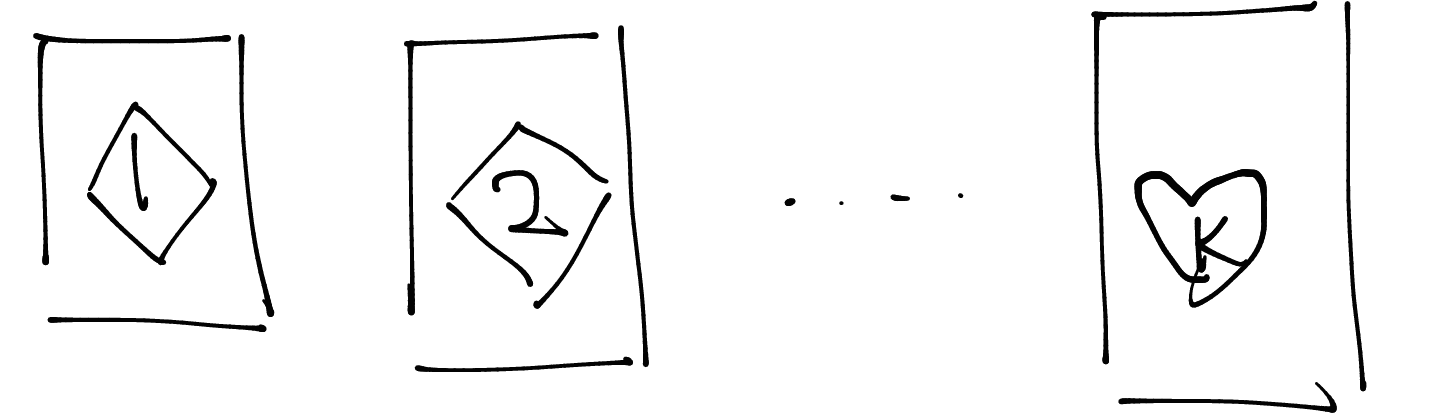
\includegraphics[width=0.6\textwidth]{img/cards.png}
    \end{figure}
   
    \item<+-> 外側からは区別できない\textbf{箱}を52個
    \begin{figure}[h]
      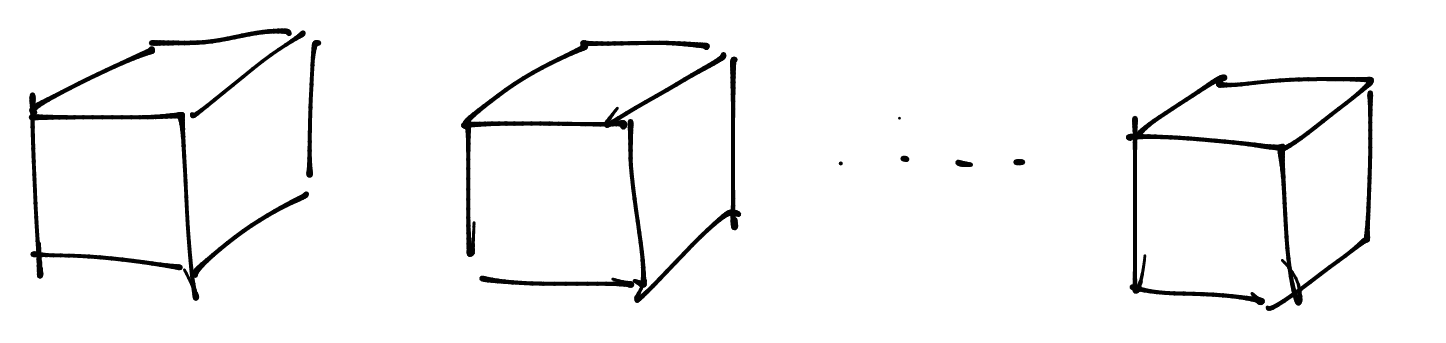
\includegraphics[width=0.6\textwidth]{img/boxes.png}
    \end{figure}
  \end{itemize}
\end{frame}

\begin{frame}
  \frametitle{用意するもの}

  \begin{itemize}
    \item<+-> アリスとボブ(Bob)
    それぞれのプレイヤーについて\textbf{南京錠}を52個ずつ
    \begin{figure}[h]
      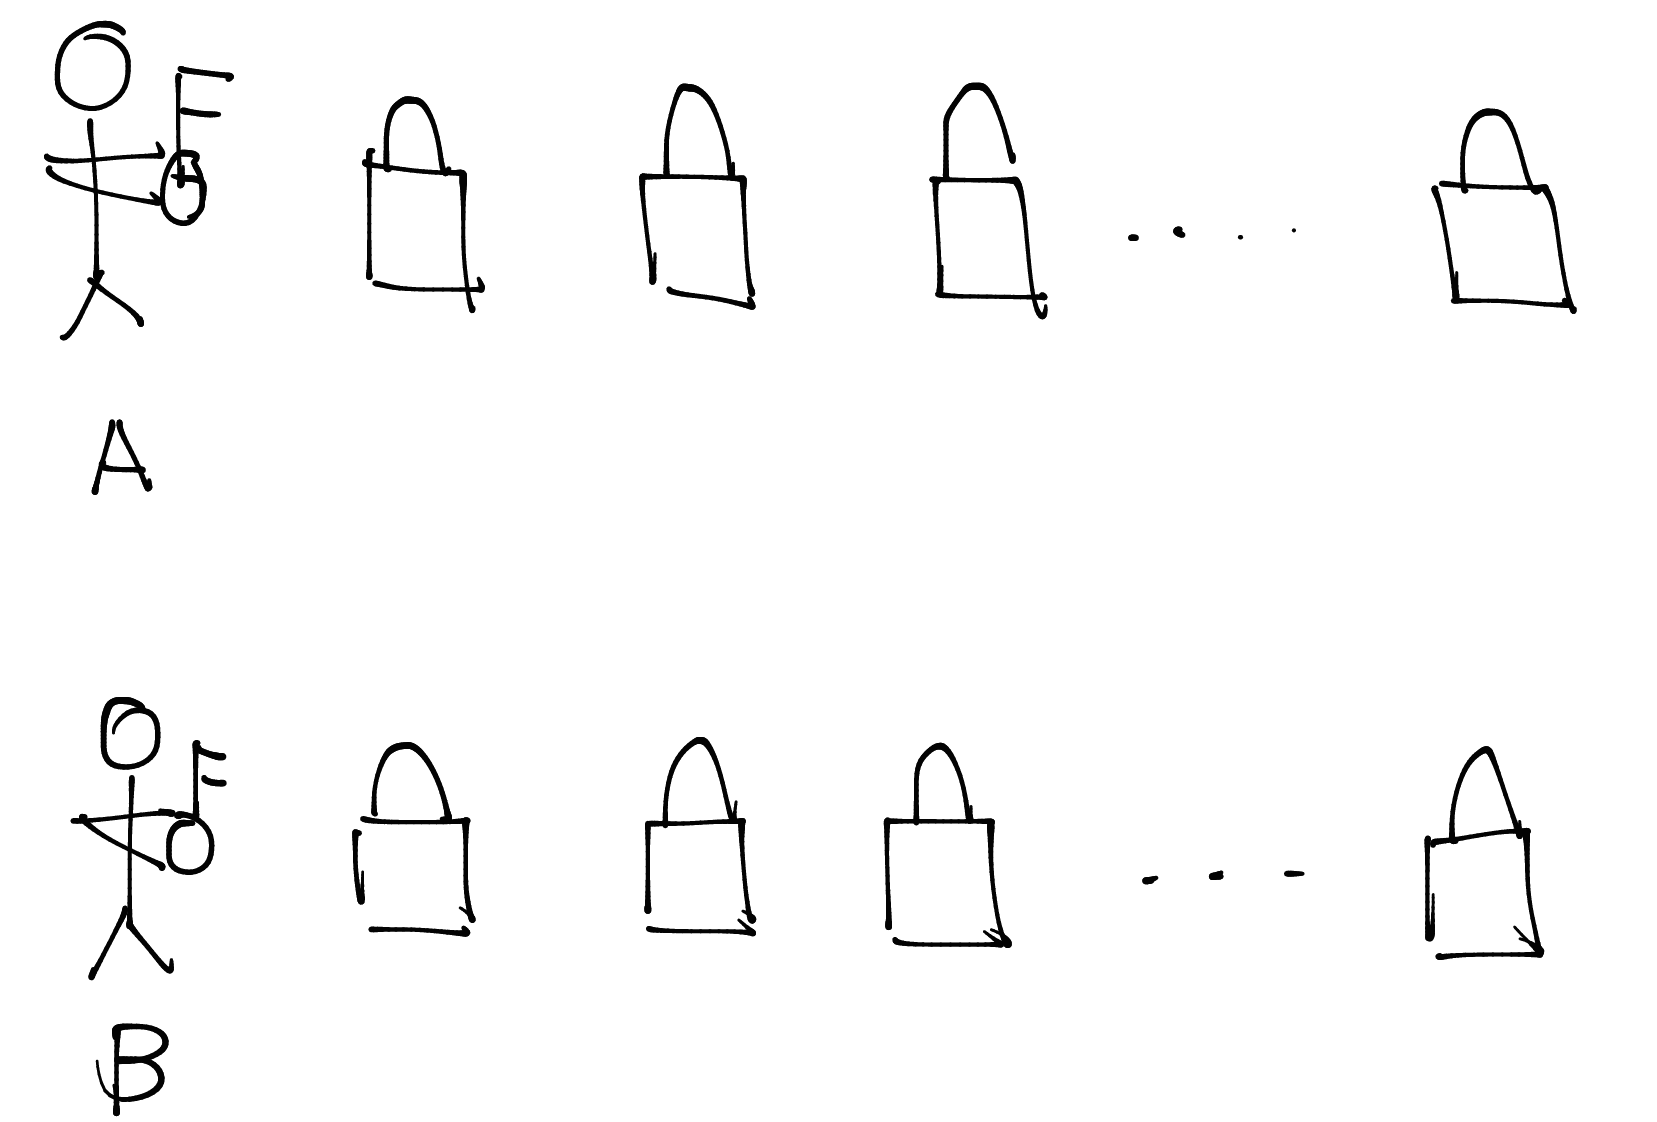
\includegraphics[width=0.6\textwidth]{img/padlocks.png}
    \end{figure}
    \begin{itemize}
      \item この南京錠は全て、アリス・ボブがそれぞれに持つ1つの鍵で開錠できる
    \end{itemize}    
  \end{itemize}
\end{frame}

\begin{frame}
  \frametitle{アリス・ボブのできること}

  \pause
  \begin{columns}
    \begin{column}{0.6\textwidth}
      \begin{itemize}
        \item<+-> 任意のカードをちょうど1枚だけ箱に入れる

        \item<+-> ちょうど1枚のカードを箱から取り出す

        \item<+-> 箱に南京錠をかける
        \begin{itemize}
          \item 南京錠は箱に任意の数つけることができる
        \end{itemize}
      \end{itemize}
    \end{column}
    \begin{column}{0.4\textwidth}
      \begin{figure}[h]
        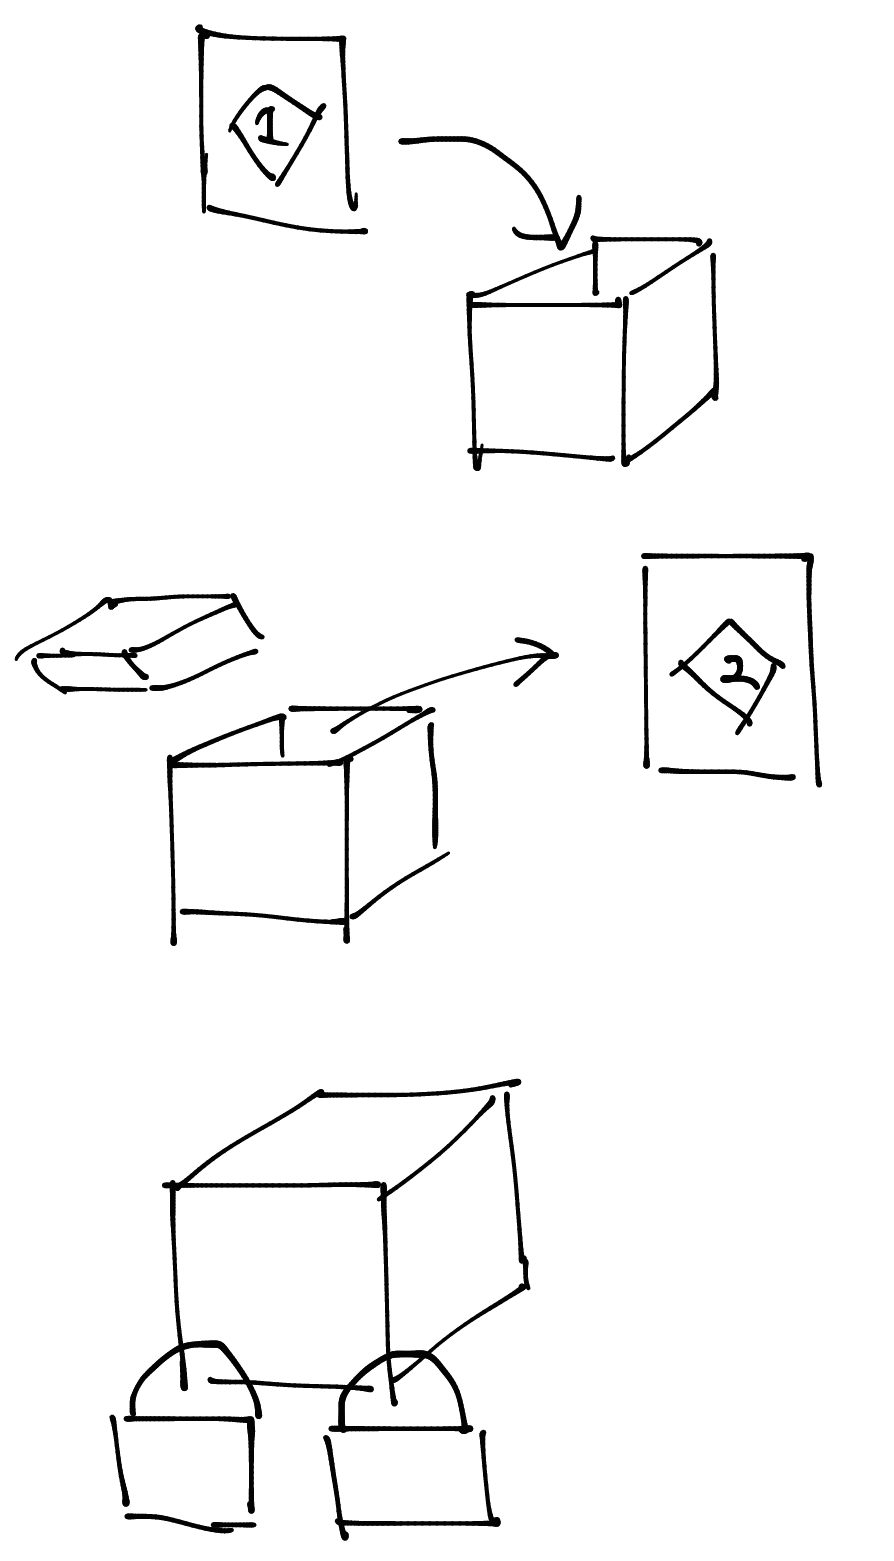
\includegraphics[height=0.8\textheight]{img/we_can.png}
      \end{figure}
    \end{column}
  \end{columns}
\end{frame}

\begin{frame}
  \frametitle{アリス・ボブのできること}

  \begin{itemize}
    \item<+-> 彼らの鍵を使って南京錠を取り外す
    \begin{figure}[h]
      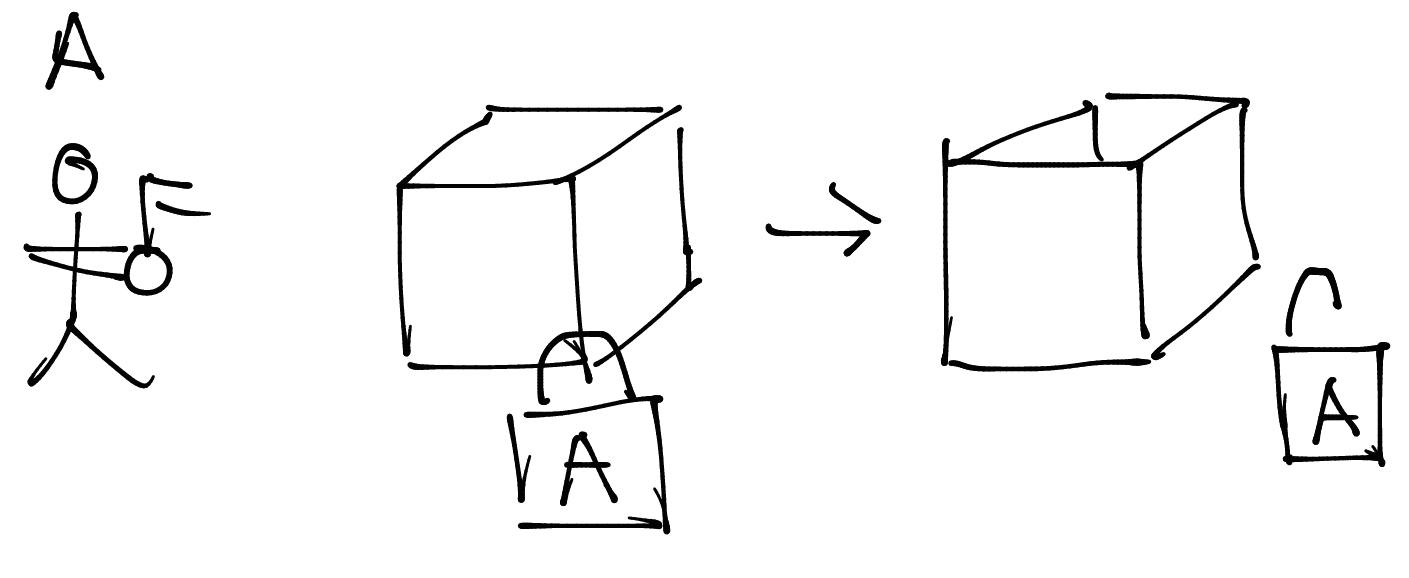
\includegraphics[width=0.7\textwidth]{img/we_can2.png}
    \end{figure}
    \begin{itemize}
      \item<+-> 南京錠が箱に複数ついている場合、
      どのような順番で開錠しても箱の中身は変化しない
    \end{itemize}
  \end{itemize}
\end{frame}

\begin{frame}
  \frametitle{アリス・ボブのできないこと}

  \pause
  \begin{itemize}
    \item<+-> \textbf{あいていない箱}の中のカードを知る
    \begin{itemize}
      \item 箱の中にあるカードの情報を知るには、
      まず箱をあける必要がある
    \end{itemize}
   
    \item<+-> あいていない箱にカードを入れる
    \item<+-> あいていない箱からカードを取り出す
    
    \item<+-> \textbf{他者の南京錠が1つでもかかった箱}を開錠し、箱をあける
    \begin{figure}[h]
      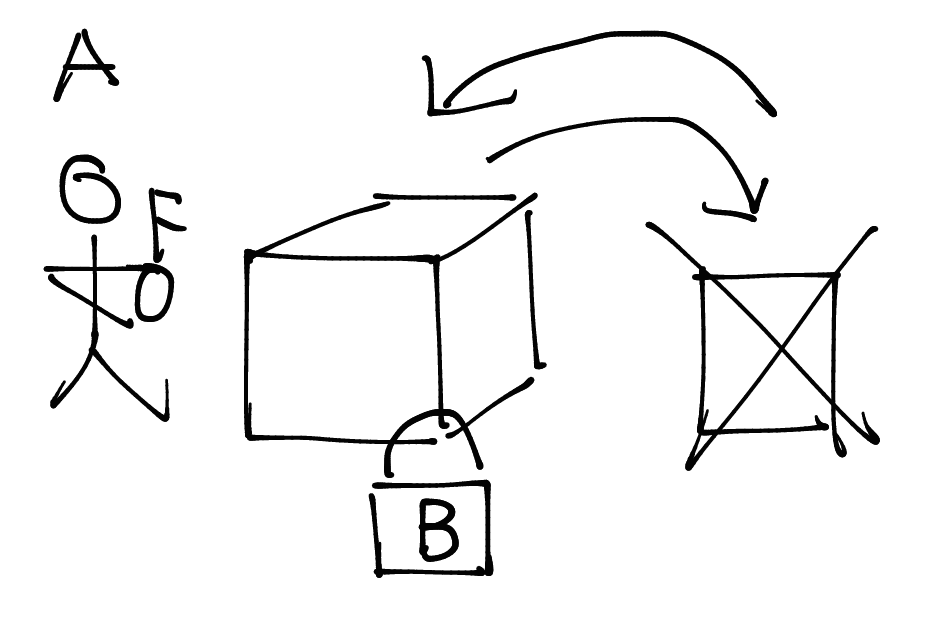
\includegraphics[width=0.6\textwidth]{img/we_can_not.png}
    \end{figure}
  \end{itemize}
\end{frame}

\section{Mental Pokerのプロトコル}

\begin{frame}

  \centering
  {\huge Mental Pokerプロトコル}

  \vspace{1em}

  ---山札づくり---
\end{frame}

\newcounter{ProtocolIndex}
\setcounter{ProtocolIndex}{1}
\newcommand*{\showIndex}{\theProtocolIndex .\;}
\newcommand*{\showAndIncrement}{%
  \showIndex%
  \stepcounter{ProtocolIndex}%
}

\begin{frame}
  \frametitle{\showAndIncrement アリスのターン}

  \begin{itemize}
    \item アリスは全ての箱に1枚ずつカードを入れ、全てにアリスの南京錠をかける
    \begin{figure}[h]
      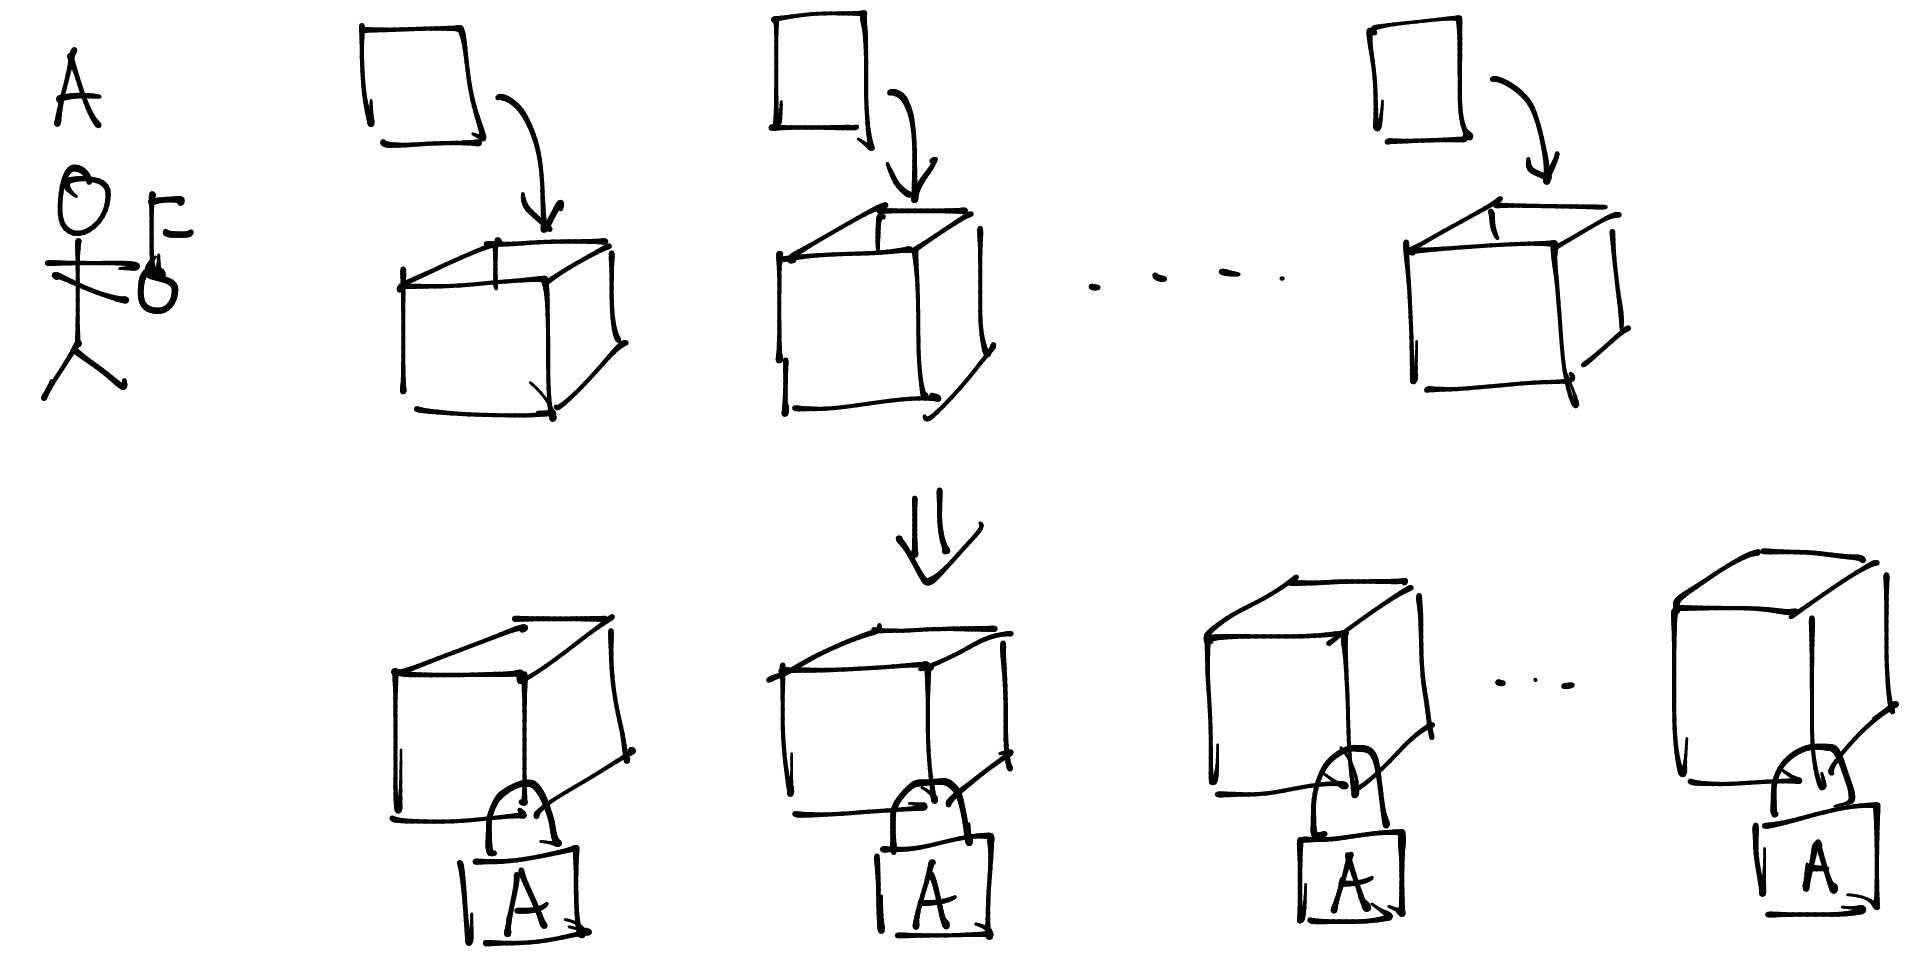
\includegraphics[width=0.8\textwidth]{img/make_deck.png}
    \end{figure}
  \end{itemize}
\end{frame}

\begin{frame}
  \frametitle{\showIndex アリスのターン}

  \begin{itemize}
    \item<+-> アリスは全ての箱をボブへ送信する
    \begin{figure}[h]
      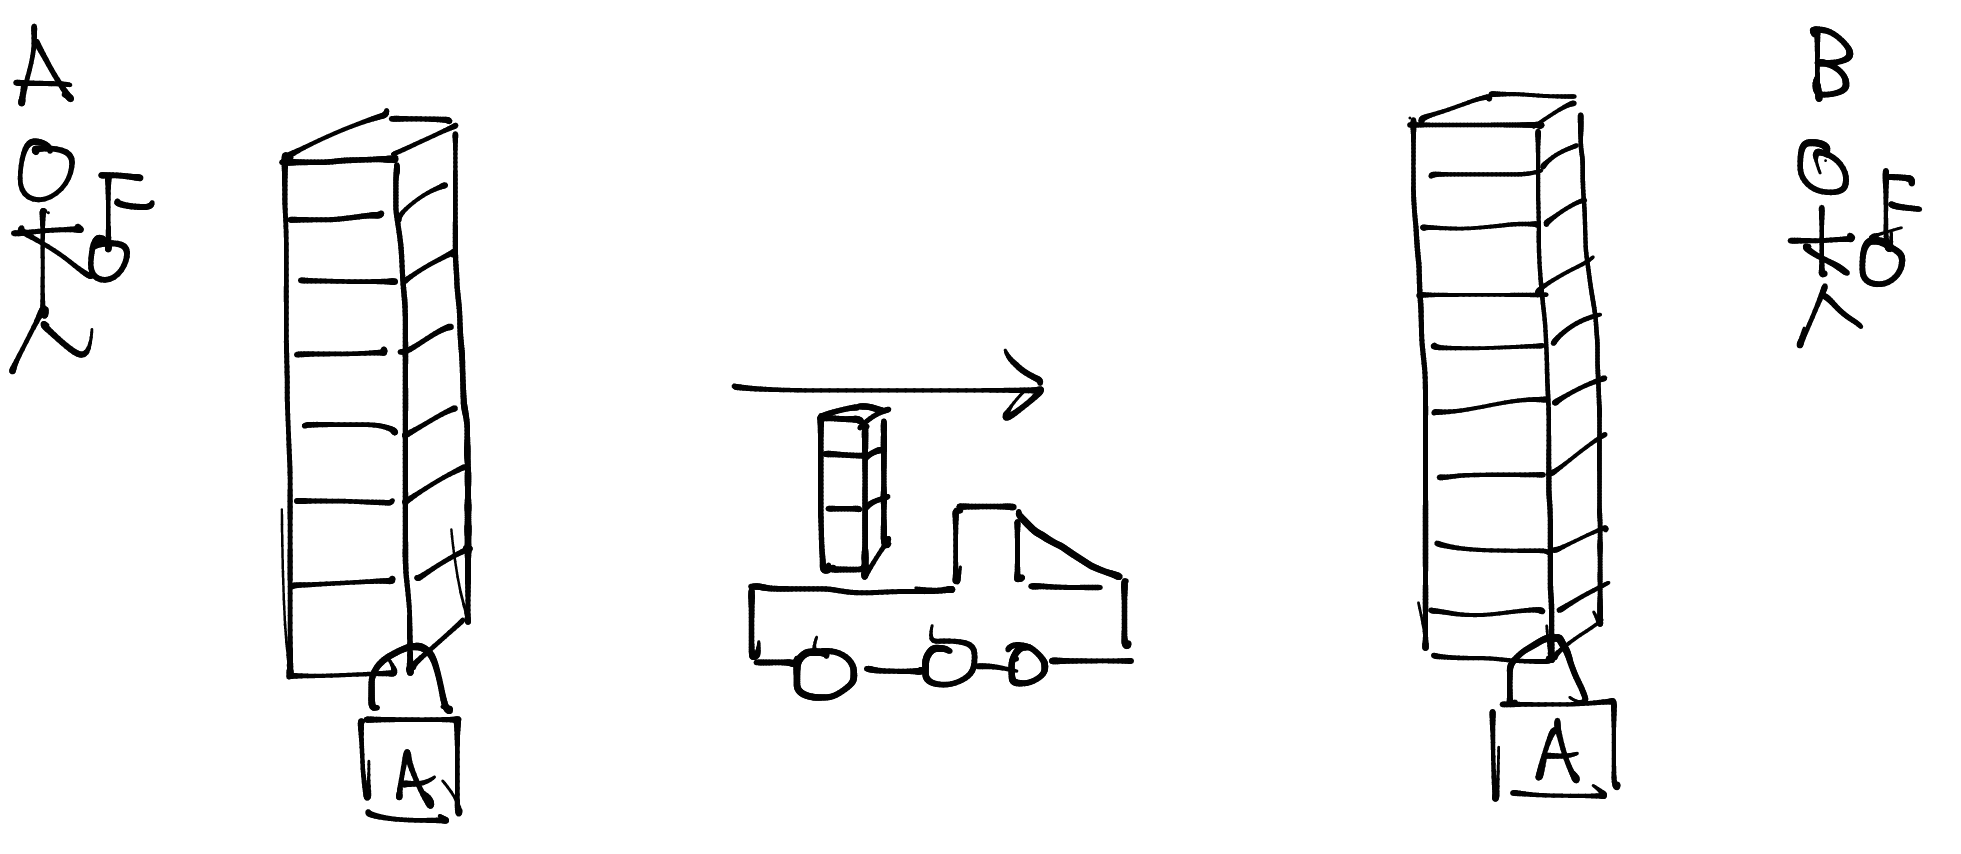
\includegraphics[width=0.9\textwidth]{img/send_to_b.png}
    \end{figure}

    \item<+-> このとき、アリスは自分で箱の中にカードを入れたので、
    カードと箱の対応を記録しておくことができる\ce{😈}
  \end{itemize}
\end{frame}

\stepcounter{ProtocolIndex}

\begin{frame}
  \frametitle{\showIndex ボブのターン}

  \begin{itemize}
    \item<+-> ボブは受け取った山札をシャッフルし、ボブの南京錠をかける
    \begin{figure}[h]
      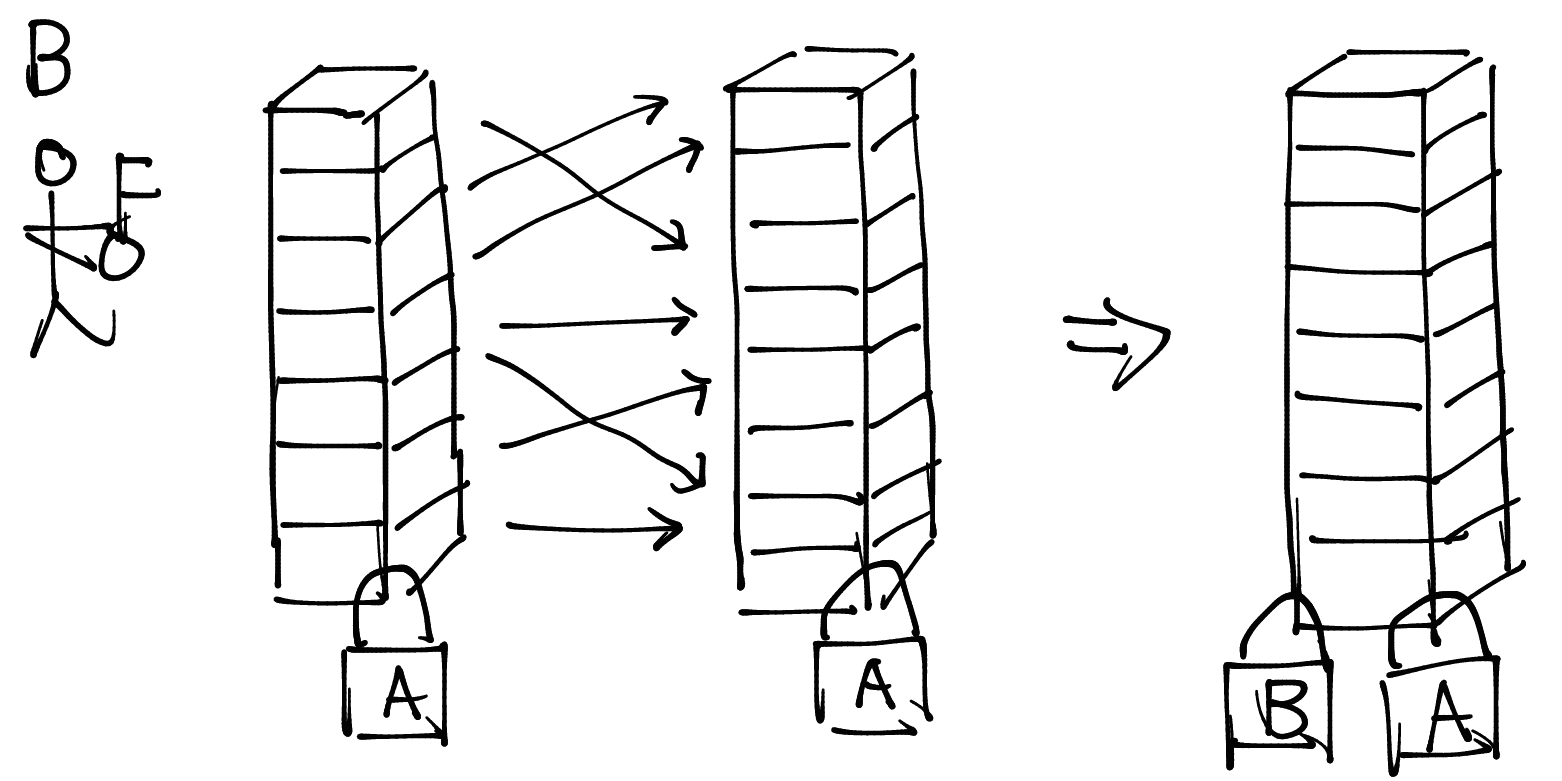
\includegraphics[width=0.75\textwidth]{img/shuffle_deck.png}
    \end{figure}

    \item<+-> ボブはアリスがどのように箱を並べたのか知らないため、
    箱の中にあるカードについて情報を得ることができない

    \item<+-> またアリスは箱の順番を記録したかもしれないが、
    ボブによってシャッフルされたため分からなくなる\ce{😇}
  \end{itemize}
\end{frame}

\stepcounter{ProtocolIndex}

\begin{frame}
  \frametitle{\showIndex ボブのターン}

  \begin{itemize}
    \item<+-> ボブは全ての箱をアリスへ送信する
    \begin{figure}[h]
      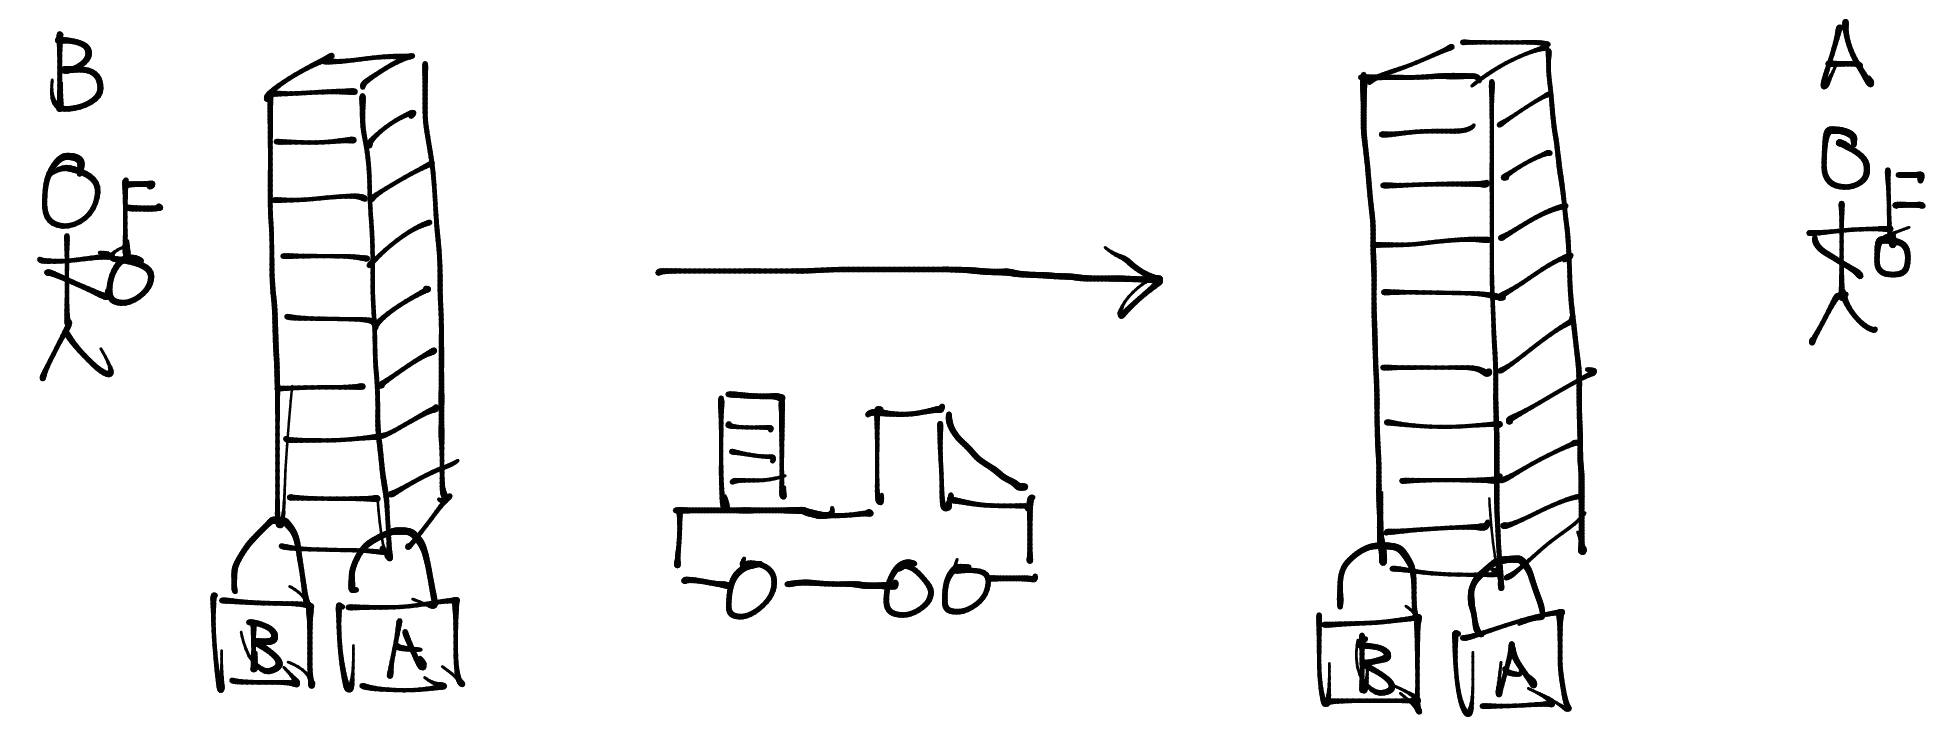
\includegraphics[width=0.8\textwidth]{img/send_to_a.png}
    \end{figure}

    \item<+-> これで山札が完成\ce{🎉}
  \end{itemize}
\end{frame}

\stepcounter{ProtocolIndex}

\begin{frame}

  \centering
  {\huge Mental Pokerプロトコル}

  \vspace{1em}

  ---初期手札のドロー\footnote[frame]{この頃の僕はポーカーのルールである「テキサスホールデム」を理解していなかったので、手札を5枚ドローする}---
\end{frame}

\begin{frame}
  \frametitle{\showAndIncrement アリスのターン}

  \begin{itemize}
    \item アリスは全ての箱の中から5個を選び、それをボブへ送信する
    \begin{figure}[h]
      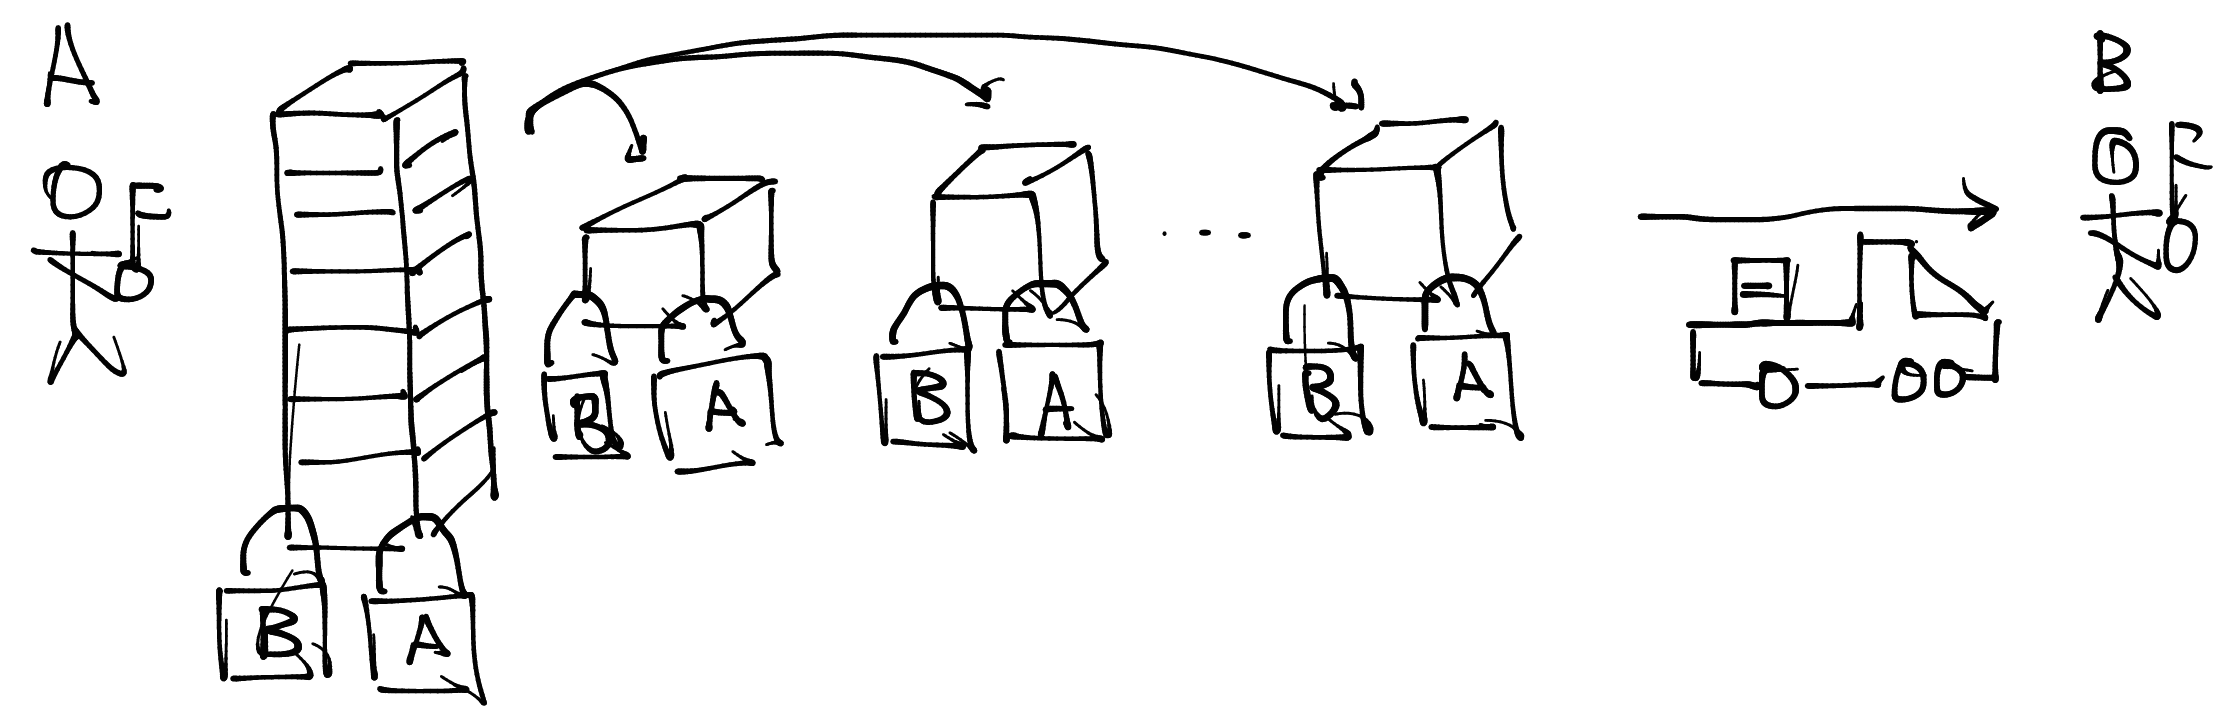
\includegraphics[width=0.9\textwidth]{img/select_boxes.png}
    \end{figure}
  \end{itemize}
\end{frame}

\begin{frame}
  \frametitle{\showIndex ボブのターン}

  \begin{itemize}
    \item<+-> ボブは受け取った5個の箱から、自分の南京錠をはずし
    箱をアリスへ送信する
    \begin{figure}[h]
      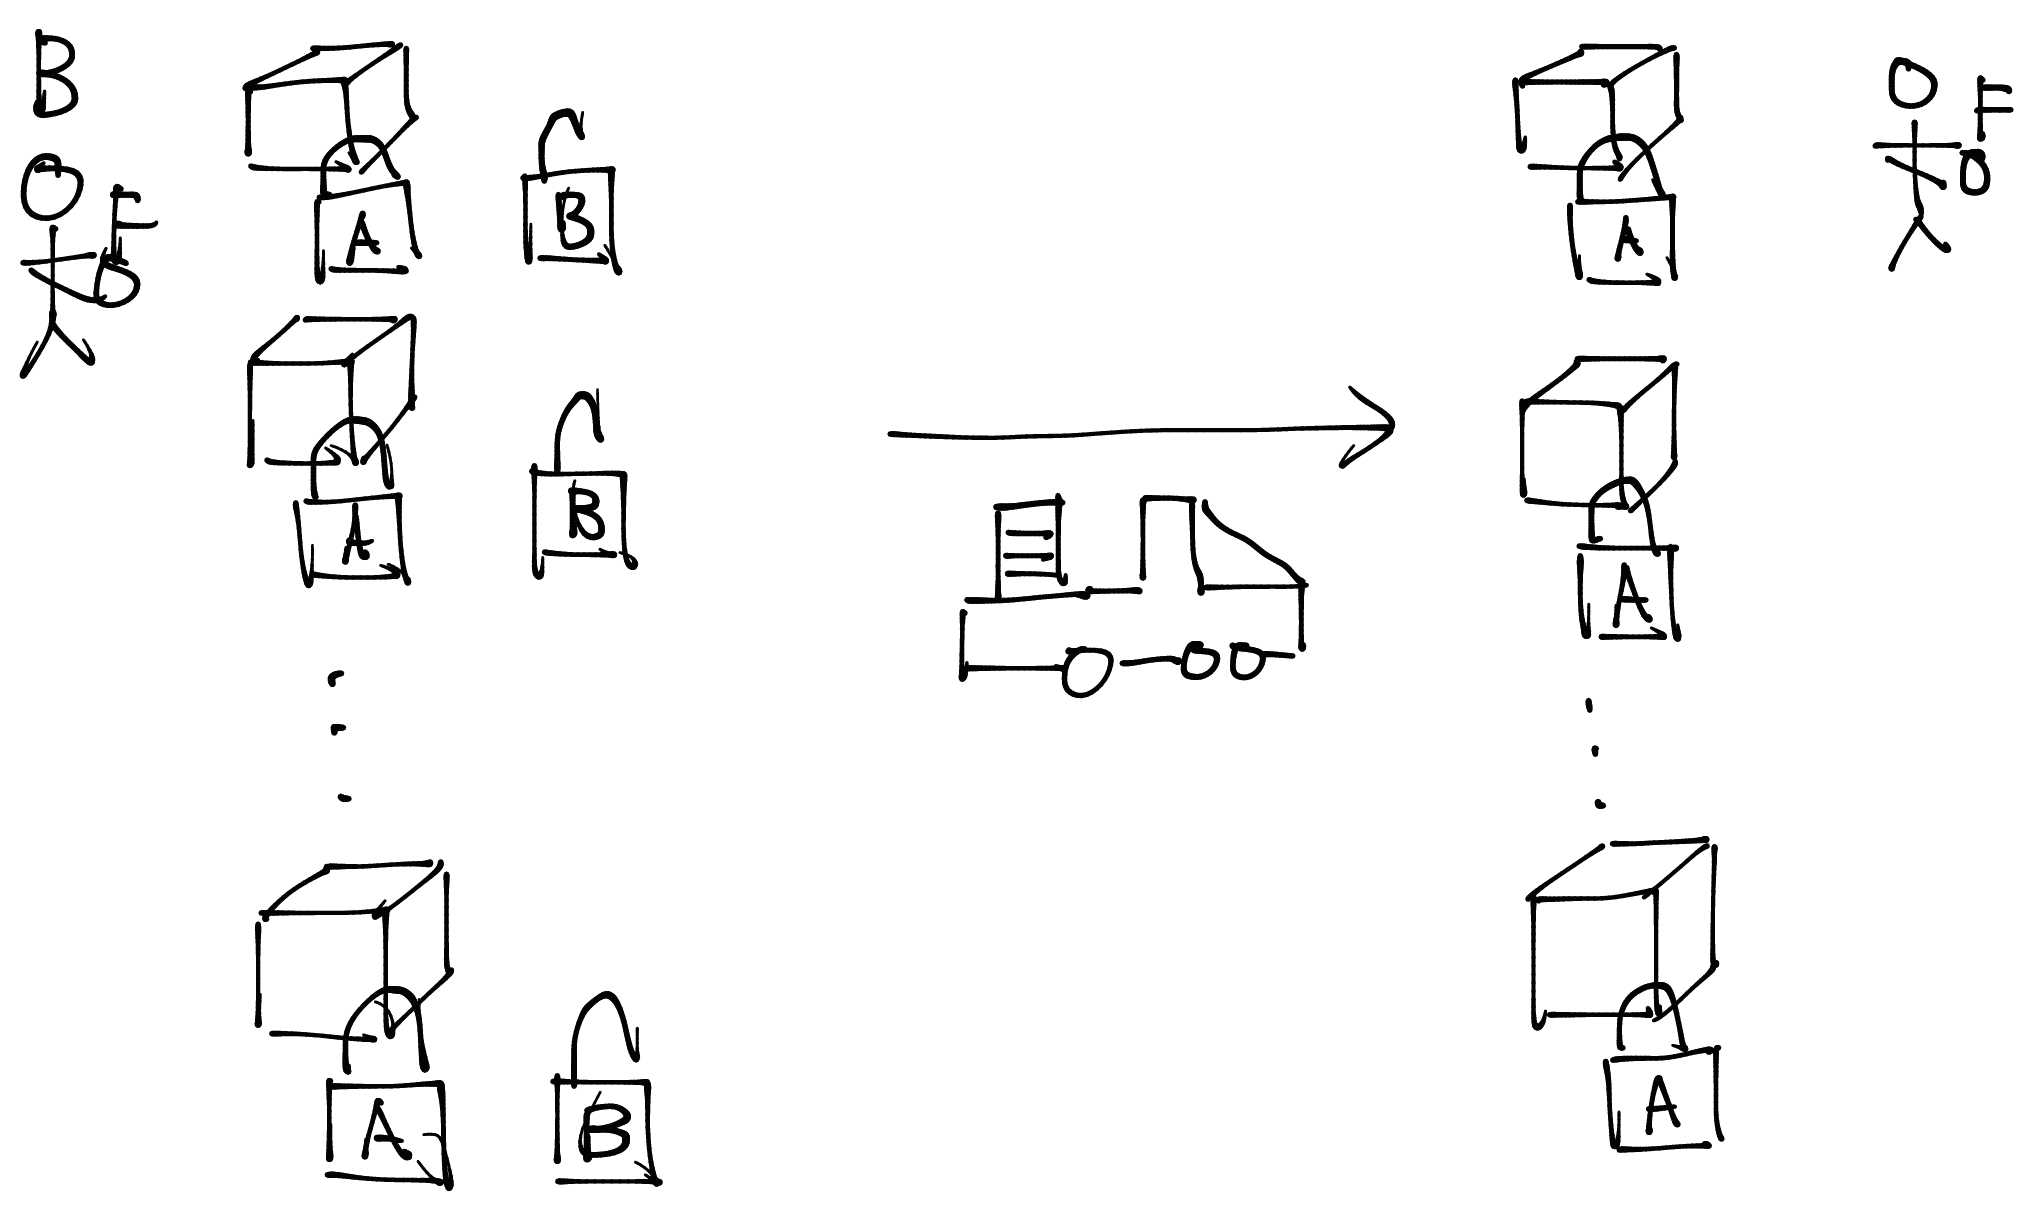
\includegraphics[width=0.8\textwidth]{img/unlock_b.png}
    \end{figure}
    \begin{itemize}
      \item<+-> このとき箱にはアリスの南京錠がまだ残っているため、
      ボブはこの5個の箱からカードを取り出すことができない
    \end{itemize}
  \end{itemize}
\end{frame}

\stepcounter{ProtocolIndex}

\begin{frame}
  \frametitle{\showIndex アリスのターン}

  \begin{itemize}
    \item<+-> アリスは受け取った5個の箱から、自分の南京錠をはずす
    \begin{figure}[h]
      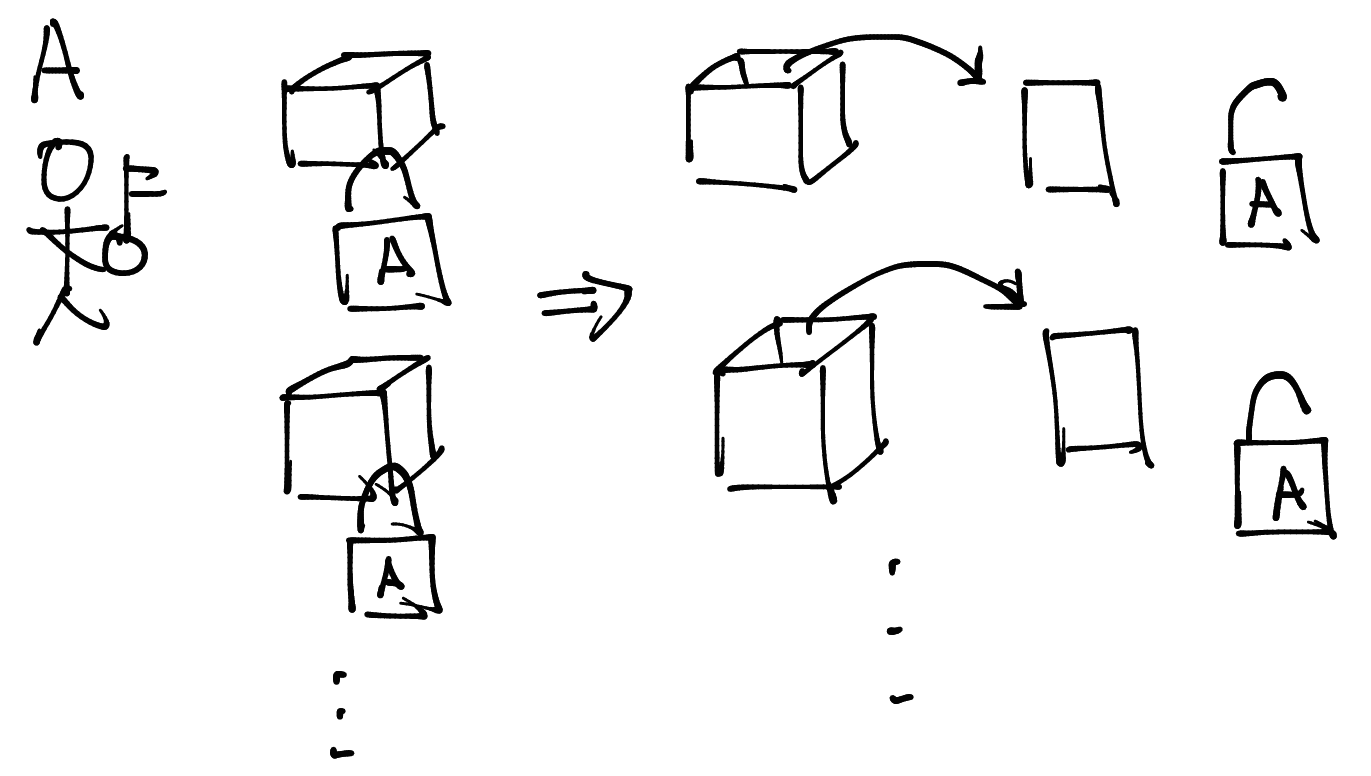
\includegraphics[width=0.85\textwidth]{img/unlock_a.png}
    \end{figure}

    \item<+-> 箱にはもう南京錠がないため、5枚のカードを得る
  \end{itemize}
\end{frame}

\stepcounter{ProtocolIndex}

\begin{frame}
  \frametitle{\showIndex ボブのターン}

  \begin{itemize}
    \item<+-> 同様の手順で、ボブも5枚のカードを得る
    \begin{figure}[h]
      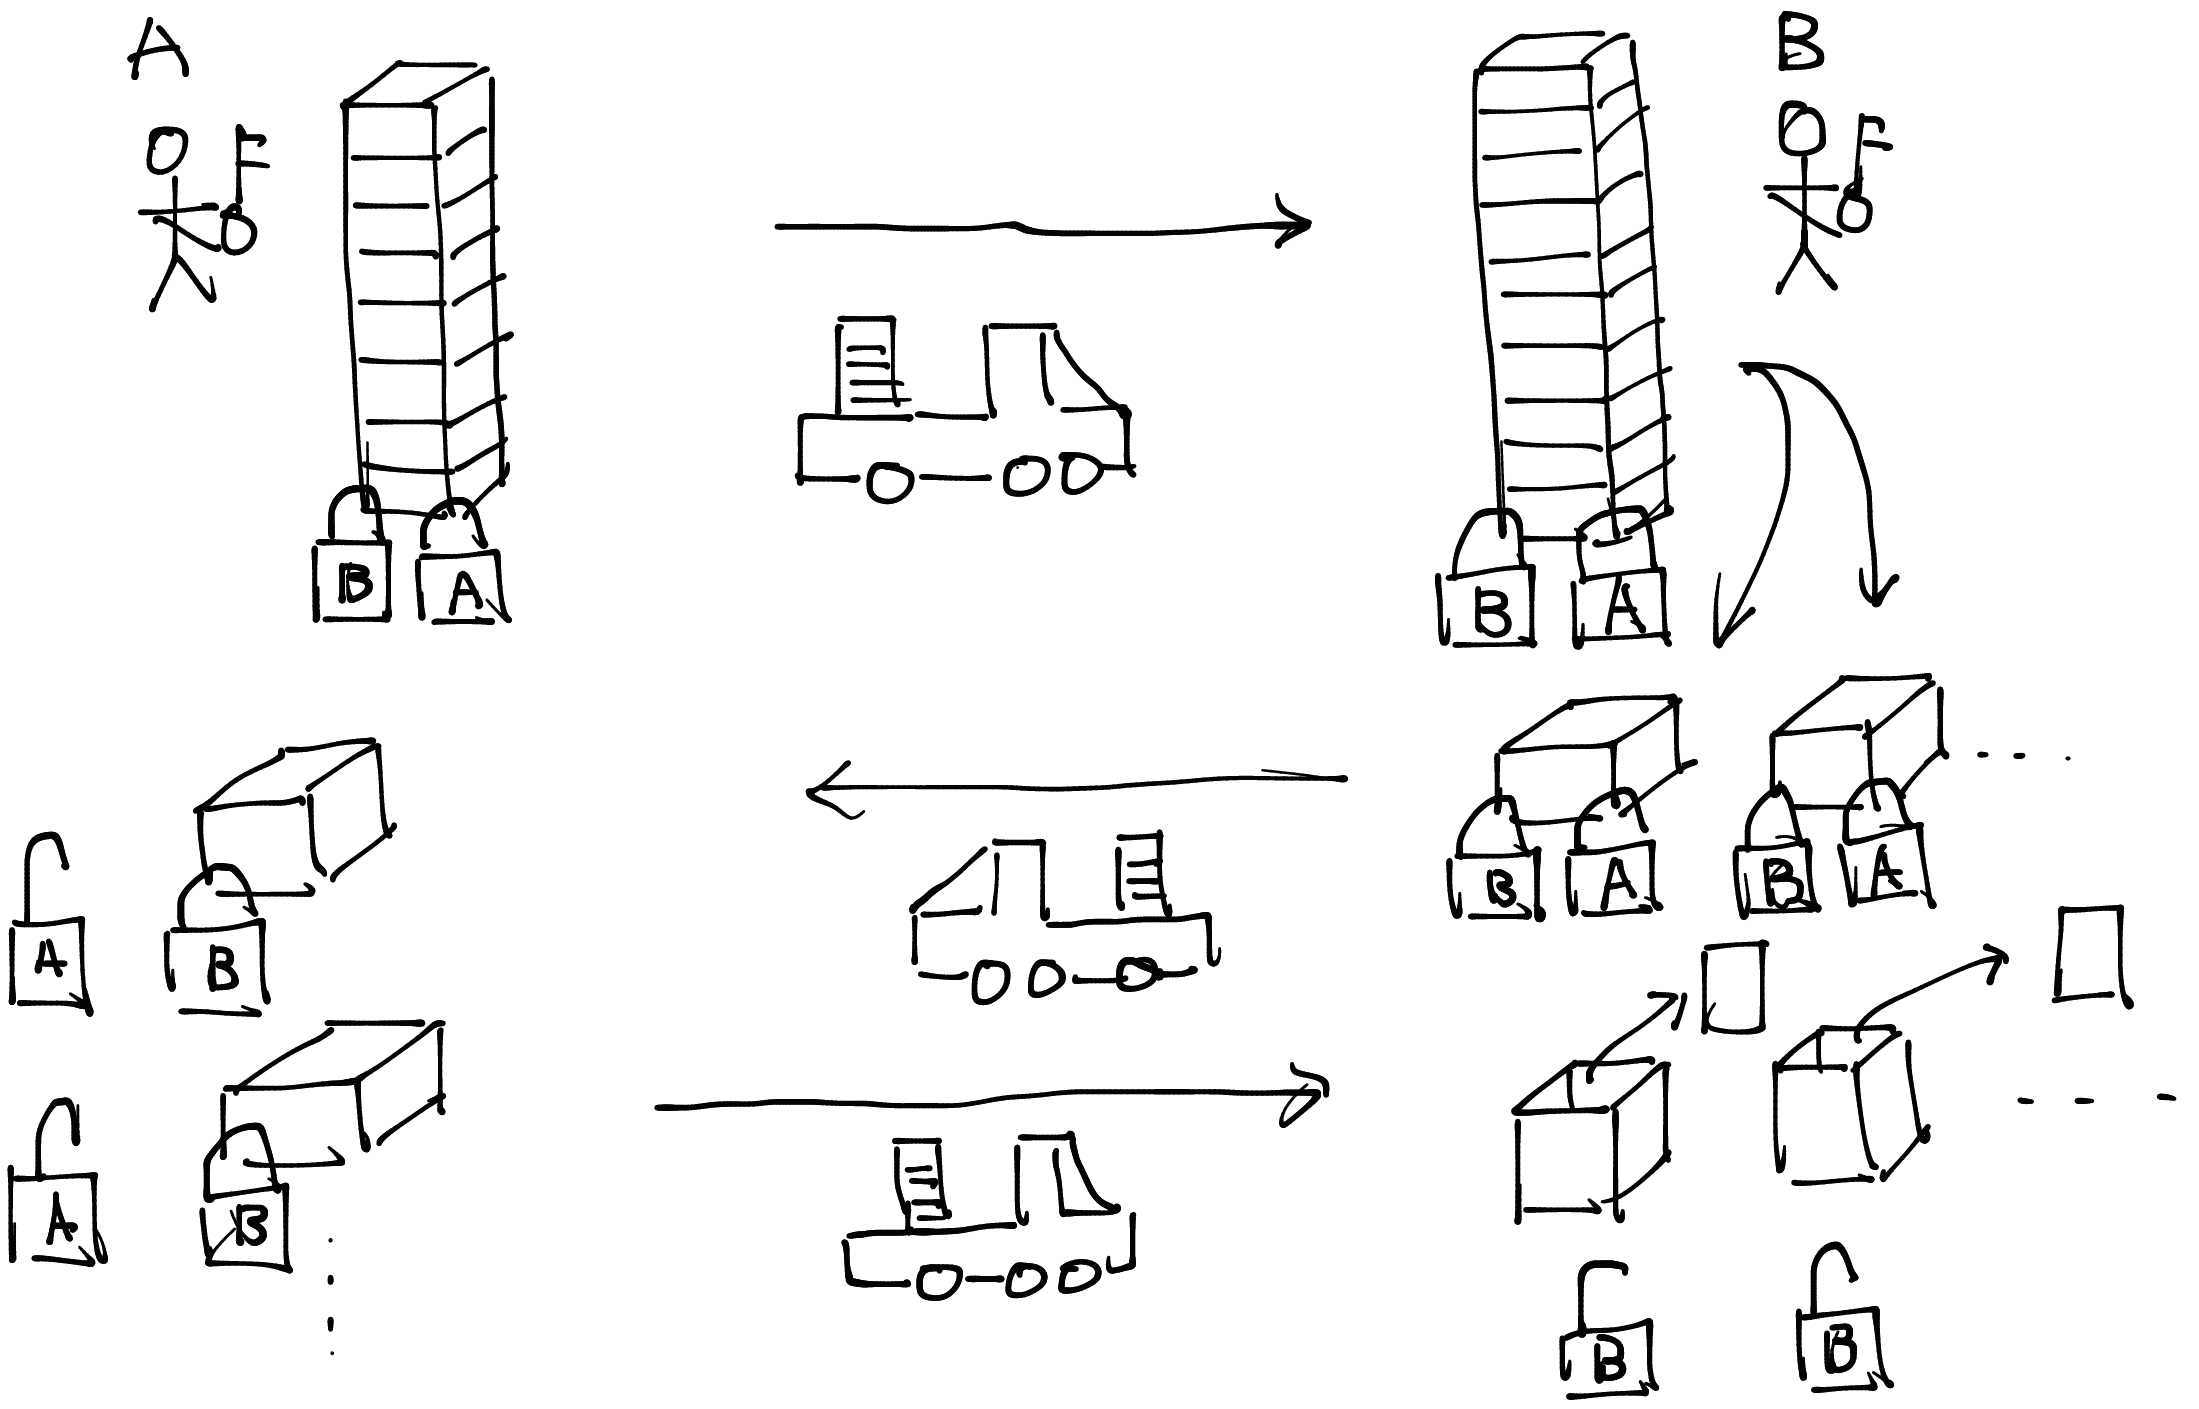
\includegraphics[width=0.85\textwidth]{img/turn_b.png}
    \end{figure}

    \item<+-> これで手札が完成\ce{🎉}
  \end{itemize}
\end{frame}

\stepcounter{ProtocolIndex}

\begin{frame}
  \frametitle{\showIndex アリス・ボブのターン}

  \begin{itemize}
    \item<+-> 後は普通にポーカーゲームをする
    \begin{itemize}
      \item カードを新たに山札からドローするときは、
      先程のプロトコルを行う
      \item カードをプレイヤー全員に公開するときは、
      単にカードを場に出せばよい
    \end{itemize}

    \item<+-> 誰かがコールするか1人を除いて全員がフォールドするなどして
    ゲームが終了したとき、参加者は全ての南京錠を開錠してカードが失くなったり、
    重複したりしていないかを確認する
    \begin{itemize}
      \item<+-> もし重複や紛失があった場合は不正とみなしゲームを無効とする
    \end{itemize}

    \item<+-> 次のゲームに進むときは、また山札作りプロトコルから
    やりなおす
  \end{itemize}
\end{frame}

\section{まとめ}

\begin{frame}
  \frametitle{まとめ}

  \pause
  \begin{itemize}
    \item<+-> このように公平な第三者なしでもポーカーができる
    \item<+-> シャッフル・ドローができれば実は多くのゲームを模倣できる
    \begin{itemize}
      \item たとえばサイコロは1から6までの数字のカードをシャッフルして1枚
      ドローする操作としてエンコードできる
    \end{itemize}

    \item<+-> 山札を最後に全て開錠しなくても不正が行われていないことを
    \textbf{ゼロ知識証明}で検証できる\cite{cmp}
    \begin{itemize}
      \item ゼロ知識証明は、たとえばいま数独パズルがあるとき、
      数独パズルの答えを誰かに教えることなく、
      自分が答えを知ってると証明する方法
    \end{itemize}

    \item<+-> 他にも\textbf{暗号通貨}と組み合せる研究\cite{Kumaresan}がある

    \item<+-> Mental Pokerを拡張してさらに色々な操作ができるようにした
    \textbf{秘密計算}は、機械学習と組み合せたりする応用\cite{ntt}がある
  \end{itemize}
\end{frame}

\section*{参考文献}

\begin{frame}
  \frametitle{参考文献}

  \bibliographystyle{junsrt_url}
  %\nocite{*}
  \bibliography{ref}
\end{frame}

\begin{frame}
  \centering
  {\Huge Thank you for your attention!}
\end{frame}

\end{document}
